\chapter{Механическая система (изменяемая и неизменяемая). Масса системы. Центр
масс и его координаты. Статические моменты массы системы относительно
полюса и плоскости. Статические моменты массы относительно центра масс и
плоскостей, проходящих через центр масс.}

Механической системой называется совокупность материальных точек. Если при
движении взаимное расположение всех материальных точек системы не изменяется, то
мы имеем дело с неизменяемой механической системой. Примером такой системы
является абсолютно твердое тело. В противном случае система называется
изменяемой. Таковыми, например, являются жидкости и газы.

Основными характеристиками механической системы являются её масса
\( \ds M = \sum_i m_i \) и центр масс \( \ds \vec{r}_c =
\frac{\sum\limits_i m_i\vec{r}_i}{M} \).

\section{Статические моменты массы системы}
Статический момент массы системы или момент инерции системы -- скалярная
физическая величина, характеризующая распределение массы тела:
\[
    I = \int \rho^2\,dm,
\]
где \( \rho \) -- расстояние от элемента тела \( dm \) до многообразия,
относительно которого измеряется момент.

В случае измерения момента относительно полюса \( \ds I = \int r^2\,dm \), в случае
плоскости \( \ds I = \int \rho^2\,dm \).

Поместив начало отсчета в центр масс имеем для момента инерции относительно
цента масс: \( I_O = \int (x^2 + y^2 + z^2)\,dm \). Для плоскостей:
\[
    I_{xOy} = \int z^2\,dm, \quad I_{yOz} = \int x^2\,dm,
    I_{xOz} = \int y^2\,dm.
\]

Нетрудно заметить, что \( I_O = I_{xOy} + I_{yOz} + I_{xOz} \).

% \begin{figure}[h!]
%     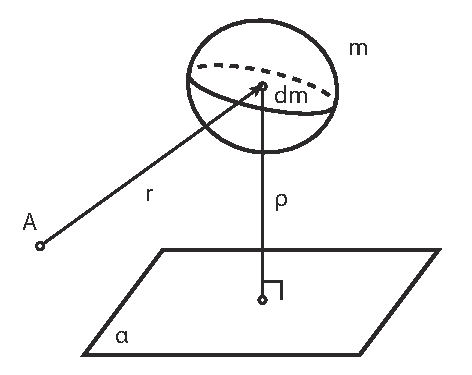
\includegraphics[width=.47\textwidth]{43_01} \hfill
%     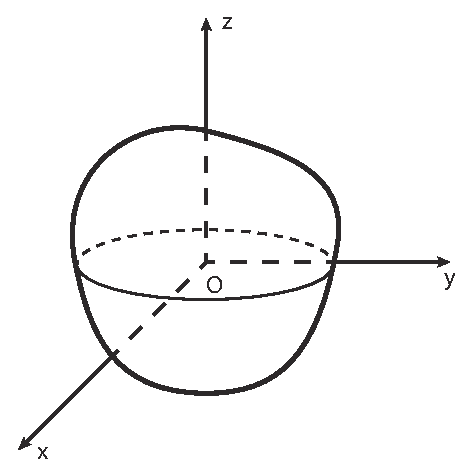
\includegraphics[width=.47\textwidth]{43_02}
%     \parbox{.47\textwidth}{\caption{Статические моменты массы относительно
%     полюса и плоскости}} \hfill
%     \parbox{.47\textwidth}{\caption{Статические моменты массы относительно
%     центра масс и плоскостей, проходящих через него}}
% \end{figure}

\newpage % ---------------------------------------------------------------------
